\chapter{Bill of Materials (BOM)\label{sec:BOM}}

A continuación, en la tabla \ref{tab:BOM} se detalla el desglose de todos los componentes necesarios para el desarrollo de este proyecto. Este documento recibe comunmente el nombre de \textit{Bill Of Materials} y permite realizar una estimación aproximada del coste del producto final.

\begin{table} [H]
\centering
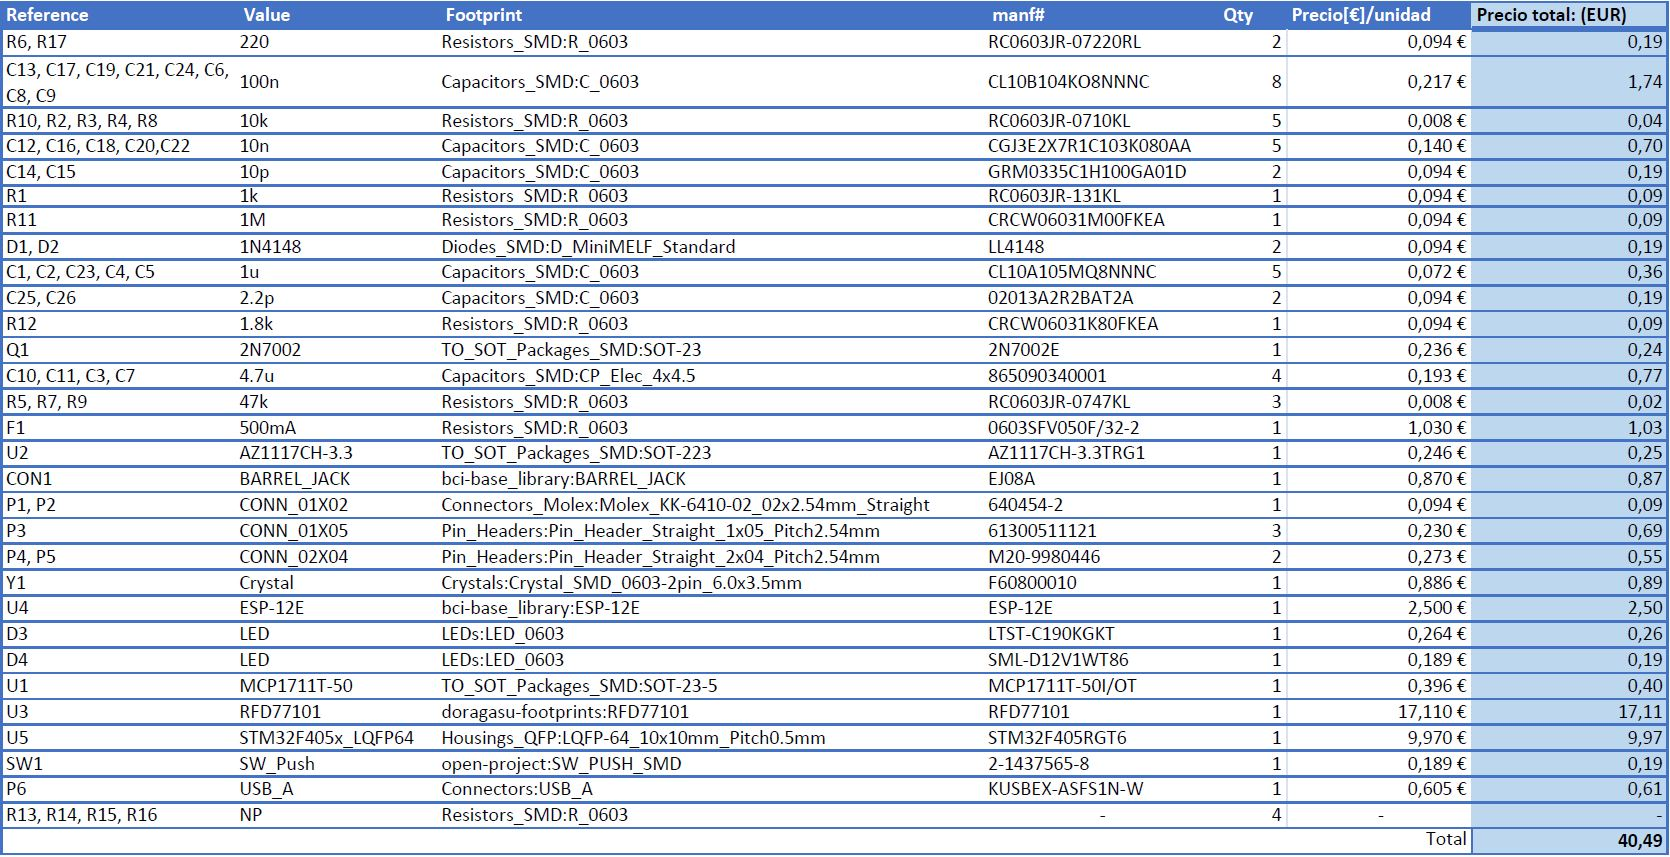
\includegraphics[width = 16cm]{BOM}
\caption{BOM - Bill of Materials}
\label{tab:BOM}
\end{table}

El coste final contando exclusivamente los materiales asciende a 40,49€. 

\clearpage

Es importante destacar que el coste de la tarjeta de procesado no sustituye al de la tarjeta de adquisición sino que lo complementa. Si se desea recrear este proyecto desde cero será imprescindible comprar todos los componentes y montar ambas tarjetas.
Teniendo en cuenta el presupuesto proyectado para la tarjeta de adquisición (97€), el de la tarjeta de procesado (40,49€) y que ciertos componentes como los módulos Bluetooth, WiFi y USB de la tarjeta de adquisición no son necesarios, \textbf{el precio final del sistema completo es inferior a los 113€}.

\chapter{Impacto ético, económico, social y ambiental\label{sec:Impacto}}

El objetivo principal de este proyecto consiste en construir un sistema capaz de realizar la adquisición de un \acrshort{EEG} con mejores prestaciones y un coste inferior al de aquellos disponibles en el mercado.

Tras cumplir este objetivo y liberar los esquemáticos diseñados se sientan unas bases que cualquier persona o institución con menos recursos puede aprovechar para construir y mejorar su propio sistema. De esta forma se amplía sensiblemente el número de personas que puede realizar investigaciones relacionadas con el estudio de un EEG y, con ello, las posibilidades de llegar a conocer en un futuro el funcionamiento de nuestro cerebro.

La investigación en este campo a corto plazo puede ayudar a la detección de patrones que estén asociados a enfermedades o incluso podría permitir realizar interfaces cerebro-ordenador (BCI) que faciliten la vida a aquellas personas que sufren algún tipo de discapacidad motora o mental.

Este proyecto cumple con la directiva RoHS (\textit{Restriction of Hazardous Substances}), es decir, las sustancias peligrosas comúnmente presentes presentes en los distintos componentes electrónicos utilizados durante la realización de este proyecto se encuentran dentro de unos márgenes definidos por la Comunidad Europea.

\begin{figure} [h]
    \centering
    
\includegraphics[width=4cm]{rohs}
    \caption{Este proyecto cumple con la directiva RoHS \cite{rohs}}
    \label{fig:rohs}
\end{figure}

\chapter{Esquemático del proyecto\label{sec:Schematic}}
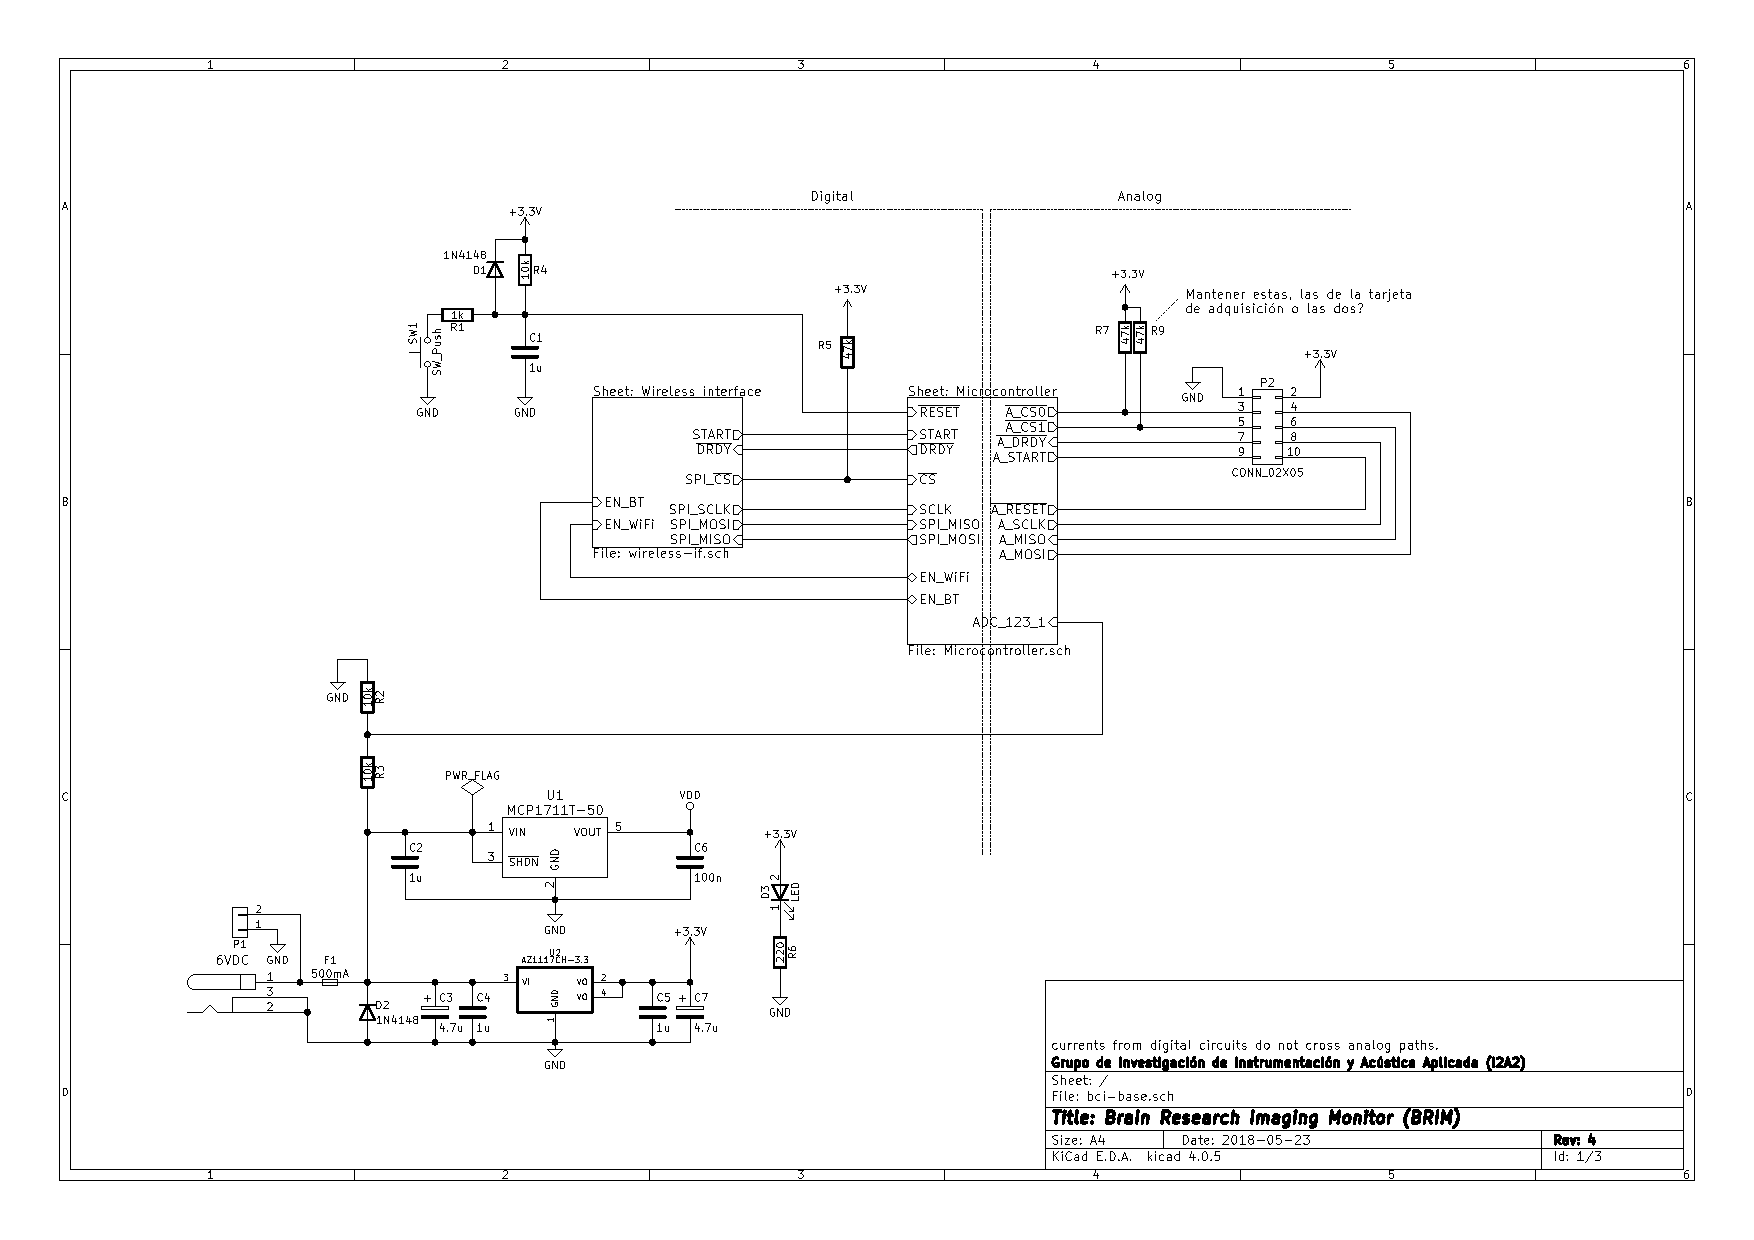
\includepdf[pages={-},angle=-90]{src/bci-base_v4.pdf} % Incluye todas las páginas de un PDF giradas -90º

\chapter{Firmware del ESP12-E\label{sec:Apendice_Code_ESP}}

Debido a la nueva normativa que permite la presentación de la memoria y documentación en formato digital se ha considerado oportuno la inclusión del código desarrollado para este proyecto en este documento, pues puede servir de referencia para futuros trabajos similares. Sin embargo, teniendo en cuenta su gran extensión, si se desea imprimir este documento se recomienda omitir la impresión de aquellos anexos relacionados con el código, especialmente el anexo \ref{sec:Apendice_Code_STM}.

Este apéndice recoge el código desarrollado para el ESP12-E. Incluye todo lo necesario para hacer de interfaz entre el ordenador y el microcontrolador STM32F4.

\begin{lstlisting}[label=algoritmo:ESP:master_fast.ino,style = STM-code,frame=single,caption=ESP:master\_fast.ino]

/*

    GPIO      Name  |   STM
   ==============================
     12       MISO  |   PA7
     13       MOSI  |   PA6
     14       SCK   |   PA5
     15       SS    |   PA4

*/
#include <SPI.h>
#include <ESP8266WiFi.h>
#include <WiFiUdp.h>

// Funciones prototipo
uint8_t read_command(uint8_t command);
void FloatArrayFromSTM(float F_array [], int N_elementos);
float floatFromSTM(void);
uint8_t String2int (String Array);
void Float2TCP (float Float_data, WiFiClient client);

char ssid[] = "SSID";
char pass[] = "PASSWORD";    

IPAddress local_IP(192,168,4,22);
IPAddress gateway(192,168,4,9);
IPAddress subnet(255,255,255,0);
IPAddress remote_IP(192,168,4,121);

// Create an instance of the server
// specify the port to listen on as an argument
WiFiServer server(80);
WiFiUDP Udp;

unsigned int localPort = 2390;      // local port to listen on


// Definición de los pines
//      Función   GPIO#
#define HSPI_CS   15
#define HSPI_CLK  14 
#define HSPI_MISO 12 
#define HSPI_MOSI 13 
#define DRDY_N    4 
#define START     5 
#define LED       2 

#define hotspot false  // hotspot = true
                    // wifi    = false
#define debug true

int i=1;

// la rutina de setup corre una vez o cuando se presiona reset
void setup() {
  Serial.begin(115200);                
  SPI.begin();

  //SPI.beginTransaction(SPISettings(16000000, MSBFIRST, SPI_MODE1));

  SPI.setClockDivider(SPI_CLOCK_DIV2); //Divides 16MHz clock by 2 to set CLK speed to 4MHz
  SPI.setDataMode(SPI_MODE1);  //clock polarity = 0; clock phase = 1 (pg. 8)
  SPI.setBitOrder(MSBFIRST);  //data format is MSB (pg. 25)  
  
  pinMode(HSPI_CS,OUTPUT);
  pinMode(HSPI_CLK,SPECIAL);
  pinMode(HSPI_MISO,SPECIAL);
  pinMode(HSPI_MOSI,SPECIAL);
  pinMode(DRDY_N,INPUT);
  pinMode(START,OUTPUT);
  pinMode(LED,OUTPUT);

  Serial.println();

  #if (hotspot == false)

  // We start by connecting to a WiFi network
  Serial.print("Connecting to ");
  Serial.println(ssid);
  WiFi.begin(ssid, pass);
  
  while (WiFi.status() != WL_CONNECTED) {
    delay(500);
    Serial.print(".");
  }
  Serial.println("");
  
  Serial.println("WiFi connected");
  Serial.println("IP address: ");
  Serial.println(WiFi.localIP());
#else

  Serial.print("Setting soft-AP configuration ... ");
  Serial.println(WiFi.softAPConfig(local_IP, gateway, subnet) ? "Ready" : "Failed!");

  Serial.print("Setting soft-AP ... ");
  Serial.println(WiFi.softAP("ESPBCI_WIFI", "Password_01", false) ? "Ready" : "Failed!");

  Serial.print("Soft-AP IP address = ");
  Serial.println(WiFi.softAPIP());

#endif

  // Start the server
  Serial.println("Starting servers");
  server.begin();
  Udp.begin(localPort);
  Serial.println("Server started");
  Serial.print("Local port: ");
  Serial.println(Udp.localPort());

}

// la rutina loop corre constantemente
void loop() {
    uint8_t command2STM = 0x02;
    uint8_t response = 0x00;
    float F_data [8];
    float F_data_array[250];
    int N_elementos = 250;
    long t1 = 0;
    int offset_configurar = 0x00;
    

  //########### Server handler #################
  // Check if a client has connected
  WiFiClient client = server.available();
  if (!client) {
    //Serial.println("No client available");
    return;
  }
  
  // Wait until the client sends some data
  Serial.println("new client");
  t1 = millis();
  while(!client.available()){
    delay(1);
    Serial.print(".");
    ESP.wdtFeed();    // Evita reinicios por watchdog
    if (millis()-t1 >= 10000){
      Serial.println("Timeout");
      return;
    }
  }
  Serial.println();
  
  // Read the first line of the request
  String req = client.readStringUntil('\r\n');
      
  #if (debug == true)    
    Serial.println(req);
  #endif

  
  // Match the request

  if (req.indexOf("Configurar") != -1)
  {
    command2STM = 0xF0;
    Serial.println("Configurar");
  }
  else if (req.indexOf("Single float") != -1)
   {
    command2STM = 0x01;
    Serial.println("Single float");
  }
  else if (req.indexOf("Float array") != -1)
    {
    command2STM = 0x02;
    Serial.println("Float array");
  }
  else{
    Serial.println("invalid request");
    client.print("invalid request\r\n");
    delay(1);
    client.flush();
    //client.stop();
    return;
  }
  

  // Prepara la respuesta para LabView
  String s = "";
  //client.setNoDelay(true);

  while (response == 0x00) // Espera a que el STM se sincronice con el ESP
  {
    response = read_command(command2STM);
    ESP.wdtFeed();    // Evita reinicios por watchdog
    Serial.println(response,HEX);
  }
   
    #if (debug == true)
      Serial.print("Comando recibido: ");
      Serial.println(response,HEX);
    #endif
    
    switch(command2STM){
      
      case 0xF0:
        #if (debug == true)
          Serial.println("CASO 0: Configurar");
        #endif
        offset_configurar = req.indexOf("Configurar");
        read_command(String2int(req.substring(offset_configurar+11,offset_configurar+19))); //Config 1
        read_command(String2int(req.substring(offset_configurar+20,offset_configurar+28))); //Config 2
        read_command(String2int(req.substring(offset_configurar+29,offset_configurar+37))); //Config 3
        read_command(String2int(req.substring(offset_configurar+38,offset_configurar+46))); //Config 4

        read_command(String2int(req.substring(offset_configurar+47,offset_configurar+55))); //Channel 1
        read_command(String2int(req.substring(offset_configurar+56,offset_configurar+64))); //Channel 2
        read_command(String2int(req.substring(offset_configurar+65,offset_configurar+73))); //Channel 3
        read_command(String2int(req.substring(offset_configurar+74,offset_configurar+82))); //Channel 4
        read_command(String2int(req.substring(offset_configurar+83,offset_configurar+91))); //Channel 5
        read_command(String2int(req.substring(offset_configurar+92,offset_configurar+100))); //Channel 6
        read_command(String2int(req.substring(offset_configurar+101,offset_configurar+109))); //Channel 7
        read_command(String2int(req.substring(offset_configurar+110,offset_configurar+118))); //Channel 8
        
        #if (debug == true)
          Serial.println("CASO 0: END");
        #endif
        
      break;
      case 0x01:    // El STM va a transmitir un dato de tipo float
        #if (debug == true)
          Serial.println("CASO 1: Single Float");
        #endif
        for (int i = 0; i<8; i++)
        {
        F_data[i] = floatFromSTM();
        Serial.println(F_data[i],7);
        }
        for (int i = 0; i<8; i++)
        {
          Float2TCP(F_data[i], client);
        }
        client.write("\r\n");   //cierra la conexión con Labview
        
        #if (debug == true)
          Serial.println("CASO 1: END");
        #endif        
      break;
      case 0x02:
        #if (debug == true)
          Serial.println("CASO 2: ARRAY");
        #endif
        t1 = millis();
        FloatArrayFromSTM(F_data_array, N_elementos);

        for (i=0; i<250; i++)
        {
         Serial.println(F_data_array[i],7);
        }
        
        for (i=0; i<250; i++)
        {
          Float2TCP(F_data_array[i], client);
          
        }
        client.write("\r\n");   //cierra la conexión con Labview

        Serial.println("END - CASO 2: ARRAY");
        
        #if (debug == true)
          Serial.println("CASO 2: END");
        #endif        
        
      break;
      default:
        #if (debug == true)
          Serial.println("Default");
        #endif
        ESP.wdtFeed();    // Evita reinicios por watchdog

        client.write("\r\n");   //cierra la conexión con Labview
        
        #if (debug == true)
          Serial.println("Default: END");
        #endif  
        
      break;
    }

  Serial.println("Client disconnected");
  
  client.flush();
  
}





uint8_t read_command(uint8_t command)
{ 
while (digitalRead(DRDY_N)!=LOW)
{
  ESP.wdtFeed();    // Evita reinicios por watchdog
  //Serial.println("Waiting for DRDY");
}

  digitalWrite(HSPI_CS, LOW);
  command = SPI.transfer(command);
  digitalWrite(HSPI_CS, HIGH);
  while(digitalRead(DRDY_N)==LOW){}  // Bloquea hasta que el ESP considera terminada la transmisión

  return command;
}

void FloatArrayFromSTM(float F_array [], int N_elementos)
{
 union miDato{
  struct
  {
    byte  b[4];     // Array de bytes de tamaño igual al tamaño de la primera variable: int = 2 bytes, float = 4 bytes
    }split;
    float fval;
  } F_recibido; 
  F_recibido.fval = 8765.4321;
  int i = 0;

while (digitalRead(DRDY_N)!=LOW)
{
  ESP.wdtFeed();    // Evita reinicios por watchdog
  //Serial.println("Waiting for DRDY");
}

long t1 = millis();
     digitalWrite(HSPI_CS, LOW);
     for (i = 0; i<N_elementos; i++)
        {
           F_recibido.split.b[0] = SPI.transfer(0b01000000);
           F_recibido.split.b[1] = SPI.transfer(0b01000000);
           F_recibido.split.b[2] = SPI.transfer(0b01000000);
           F_recibido.split.b[3] = SPI.transfer(0b01000000);
           
           F_array[i]=F_recibido.fval;
        }

Serial.println(millis()-t1);
        
     digitalWrite(HSPI_CS, HIGH);
     
while (digitalRead(DRDY_N)==LOW)
{
  ESP.wdtFeed();    // Evita reinicios por watchdog
} 
 // Espera a que DRDY levante, significa que se ha acabado el bucle.
 // Bloquea el micro pero asegura que no entra más de una vez
      
     if (digitalRead(LED)==1)
       digitalWrite(LED,LOW);
     else
       digitalWrite(LED,HIGH);     
}

float floatFromSTM(void)
{
  union miDato{
    struct
    {
      byte  b[4];     // Array de bytes de tamaño igual al tamaño de la primera variable: int = 2 bytes, float = 4 bytes
    }split;
    float fval;
  } F_recibido;
   
  F_recibido.fval = 8765.4321;
  int i = 0;

  digitalWrite(HSPI_CS, LOW);
  while (digitalRead(DRDY_N)!=LOW)
  {
    ESP.wdtFeed();    // Evita reinicios por watchdog
    //Serial.println("Waiting for DRDY");
  }
  F_recibido.split.b[0] = SPI.transfer(0b01000000);
  F_recibido.split.b[1] = SPI.transfer(0b01000000);
  F_recibido.split.b[2] = SPI.transfer(0b01000000);
  F_recibido.split.b[3] = SPI.transfer(0b01000000);
  
  digitalWrite(HSPI_CS, HIGH);
       
  while (digitalRead(DRDY_N)==LOW)
  {
    ESP.wdtFeed();    // Evita reinicios por watchdog
  } 
  // Espera a que DRDY levante, significa que se ha acabado el bucle.
  // Bloquea el micro pero asegura que no entra más de una vez
      
  if (digitalRead(LED)==1)
   digitalWrite(LED,LOW);
  else
   digitalWrite(LED,HIGH);   

  return F_recibido.fval;
}

uint8_t String2int (String Array)
{
  uint8_t output = 0x00;
  for (int i = 0; i < 8; i++)
    bitWrite(output, i, bitRead(Array[7-i], 0));
  
  return output;
}

void Float2TCP (float Float_data, WiFiClient client)
{
  union miDato{
  struct
  {
    byte  b[4];     // Array de bytes de tamaño igual al tamaño de la primera variable: int = 2 bytes, float = 4 bytes
  }split;
  float fval;
} F_recibido;

  F_recibido.fval = Float_data;
 
  client.write(F_recibido.split.b[3]); // Envía la respuesta a LabView
  client.write(F_recibido.split.b[2]); // Envía la respuesta a LabView
  client.write(F_recibido.split.b[1]); // Envía la respuesta a LabView
  client.write(F_recibido.split.b[0]); // Envía la respuesta a LabView*/
}
\end{lstlisting}

\chapter{Firmware del STM32F4\label{sec:Apendice_Code_STM}}

A continuación se incluye el firmware desarrollado para el microcontrolador STM32F4, mostrando los ficheros más importantes y obviando aquellos generados de forma automática o presentes en las librerías aunque estos hayan sido de utilidad.

\begin{lstlisting}[label=algoritmo:STM32F4:main.c,style = STM-code,frame=single,caption=STM32F4:main.c]
/* 
  ************************************************
  * File Name          : main.c
  * Description        : Main program body
  ************************************************
  * This notice applies to any and all portions of this file
  * that are not between comment pairs USER CODE BEGIN and
  * USER CODE END. Other portions of this file, whether 
  * inserted by the user or by software development tools
  * are owned by their respective copyright owners.
  *
  * Copyright (c) 2018 STMicroelectronics International N.V. 
  * All rights reserved.
  *
  * Redistribution and use in source and binary forms, with or without 
  * modification, are permitted, provided that the following conditions are met:
  *
  * 1. Redistribution of source code must retain the above copyright notice, 
  *    this list of conditions and the following disclaimer.
  * 2. Redistributions in binary form must reproduce the above copyright notice,
  *    this list of conditions and the following disclaimer in the documentation
  *    and/or other materials provided with the distribution.
  * 3. Neither the name of STMicroelectronics nor the names of other 
  *    contributors to this software may be used to endorse or promote products 
  *    derived from this software without specific written permission.
  * 4. This software, including modifications and/or derivative works of this 
  *    software, must execute solely and exclusively on microcontroller or
  *    microprocessor devices manufactured by or for STMicroelectronics.
  * 5. Redistribution and use of this software other than as permitted under 
  *    this license is void and will automatically terminate your rights under 
  *    this license. 
  *
  * THIS SOFTWARE IS PROVIDED BY STMICROELECTRONICS AND CONTRIBUTORS "AS IS" 
  * AND ANY EXPRESS, IMPLIED OR STATUTORY WARRANTIES, INCLUDING, BUT NOT 
  * LIMITED TO, THE IMPLIED WARRANTIES OF MERCHANTABILITY, FITNESS FOR A 
  * PARTICULAR PURPOSE AND NON-INFRINGEMENT OF THIRD PARTY INTELLECTUAL PROPERTY
  * RIGHTS ARE DISCLAIMED TO THE FULLEST EXTENT PERMITTED BY LAW. IN NO EVENT 
  * SHALL STMICROELECTRONICS OR CONTRIBUTORS BE LIABLE FOR ANY DIRECT, INDIRECT,
  * INCIDENTAL, SPECIAL, EXEMPLARY, OR CONSEQUENTIAL DAMAGES (INCLUDING, BUT NOT
  * LIMITED TO, PROCUREMENT OF SUBSTITUTE GOODS OR SERVICES; LOSS OF USE, DATA, 
  * OR PROFITS; OR BUSINESS INTERRUPTION) HOWEVER CAUSED AND ON ANY THEORY OF 
  * LIABILITY, WHETHER IN CONTRACT, STRICT LIABILITY, OR TORT (INCLUDING 
  * NEGLIGENCE OR OTHERWISE) ARISING IN ANY WAY OUT OF THE USE OF THIS SOFTWARE,
  * EVEN IF ADVISED OF THE POSSIBILITY OF SUCH DAMAGE.
  *
  ************************************************
  */

/* Includes --------------------------------------*/
#include "main.h"
#include "stm32f4xx_hal.h"
#include "usb_host.h"
/* USER CODE BEGIN Includes */

#include "util.h"
#include "ADS1299.h"
#include "stdbool.h"
#include <stdlib.h>

// Includes y defines relacionados con el filtro FIR
#include "arm_math.h"
#include "math_helper.h"

/* USER CODE END Includes */

/* Private variables ------------------------------*/
ADC_HandleTypeDef hadc1;

SPI_HandleTypeDef hspi1;
SPI_HandleTypeDef hspi2;

UART_HandleTypeDef huart4;

/* USER CODE BEGIN PV */
/* Private variables -------------------------------*/

/* USER CODE END PV */

/* Private function prototypes ---------------------*/
void SystemClock_Config(void);
static void MX_GPIO_Init(void);
static void MX_SPI1_Init(void);
static void MX_SPI2_Init(void);
static void MX_ADC1_Init(void);
static void MX_UART4_Init(void);
void MX_USB_HOST_Process(void);

/* USER CODE BEGIN PFP */
/* Private function prototypes ---------------------*/

	uint8_t commandFromESP (uint8_t command, SPI_HandleTypeDef *SPI);
	void float2ESP (float32_t data2ESP, SPI_HandleTypeDef *SPI);
	void floatArray2ESP ( float32_t data2ESP_array[], int N_elementos, SPI_HandleTypeDef *SPI, UART_HandleTypeDef *huart4);

/* USER CODE END PFP */

/* USER CODE BEGIN 0 */

// global variables
unsigned long blink_interval_millis;
float32_t channel_1 [LENGTH_SAMPLES];
float32_t channel_2 [LENGTH_SAMPLES];
float32_t channel_3 [LENGTH_SAMPLES];
float32_t channel_4 [LENGTH_SAMPLES];
float32_t channel_5 [LENGTH_SAMPLES];
float32_t channel_6 [LENGTH_SAMPLES];
float32_t channel_7 [LENGTH_SAMPLES];
float32_t channel_8 [LENGTH_SAMPLES];

bool wait = false;
uint8_t bucle=1;
uint8_t k = 0;
int icanal=1;
int i;
bool acabar = false;
bool Data_ready = true;
uint8_t comando_temp = 0x00;

uint8_t data[27];

uint8_t command = 0x00;

int channel = 1;

float32_t data2ESP = 1234.5678;

bool shared_negative_electrode = true;

/* -------------------------------------------------
 * Declare Test output buffer
 * -------------------------------------------------*/
static float32_t testOutput[LENGTH_SAMPLES];
/* -------------------------------------------------
 * Declare State buffer of size (numTaps + blockSize - 1)
 * -------------------------------------------------*/
static float32_t firStateF32[BLOCK_SIZE + NUM_TAPS - 1];
/* -------------------------------------------------
** FIR Coefficients buffer generated using fir1() MATLAB function.
** fir1(28, 6/24)
** -------------------------------------------------*/

const float32_t firCoeffs32[NUM_TAPS] = {-0.0138029831773458, 0.0395399929599544, 0.0428349923732840, -0.0175674331348036, -0.0605461382912526, -0.0197781448960783, 0.0543574323501128, 0.0566917462875556, -0.0224447398190889, -0.0748391427030912, -0.0236934079009084, 0.0631991587299459, 0.0640421490722732, -0.0246563468927641, 0.920000000000000, -0.0246563468927641, 0.0640421490722732, 0.0631991587299459, -0.0236934079009084, -0.0748391427030912, -0.0224447398190889, 0.0566917462875556, 0.0543574323501128, -0.0197781448960783, -0.0605461382912526, -0.0175674331348036, 0.0428349923732840, 0.0395399929599544, -0.0138029831773458};

/* ------------------------------------------------------------------
 * Global variables for FIR LPF Example
 * ------------------------------------------------------------------- */
uint32_t blockSize = BLOCK_SIZE;
uint32_t numBlocks = LENGTH_SAMPLES/BLOCK_SIZE;
float32_t  snr;
	
// Inicialización de todas las variables relacionadas con el filtrado
	int i;
  arm_fir_instance_f32 S;
  arm_status status;
  float32_t  *inputF32 	= &channel_1[0];			// Definición del puntero de la señal a filtrar.
	float32_t  *outputF32 = &testOutput[0];			// Definición del puntero de la señal filtrada.

/* USER CODE END 0 */

int main(void)
{

  /* USER CODE BEGIN 1 */
	
  /* USER CODE END 1 */

  /* MCU Configuration----------------------------------------------------------*/

  /* Reset of all peripherals, Initializes the Flash interface and the Systick. */
  HAL_Init();

  /* USER CODE BEGIN Init */

	
  /* USER CODE END Init */

  /* Configure the system clock */
  SystemClock_Config();

  /* USER CODE BEGIN SysInit */
	
		
  /* USER CODE END SysInit */

  /* Initialize all configured peripherals */
  MX_GPIO_Init();
  MX_SPI1_Init();
  MX_SPI2_Init();
  MX_ADC1_Init();
  MX_UART4_Init();
  MX_USB_HOST_Init();

  /* USER CODE BEGIN 2 */
	
	//Inicialización del estado de ciertos pines
	
	HAL_GPIO_WritePin(DRDY_N_GPIO_Port,DRDY_N_Pin, GPIO_PIN_SET);
	HAL_GPIO_WritePin(LED_GPIO_Port,LED_Pin, GPIO_PIN_SET);
	HAL_GPIO_WritePin(A_START_GPIO_Port, A_START_Pin, GPIO_PIN_SET);

	// Reiniciamos el ESP12-E y lo dejamos habilitado
	
	HAL_GPIO_WritePin(EN_WIFI_GPIO_Port, EN_WIFI_Pin, GPIO_PIN_RESET);
	HAL_Delay(100);
	HAL_GPIO_WritePin(EN_WIFI_GPIO_Port, EN_WIFI_Pin, GPIO_PIN_SET);

	// Parpadeo del LED del ADS y el STM para comprobar si han arrancado bien
	
	HAL_GPIO_WritePin(LED_GPIO_Port,LED_Pin, GPIO_PIN_RESET); 	//LED ON
	adc_wreg(GPIO, 0x1C, &hspi2);				// Led 1 on, led 2 off
	HAL_Delay(500);
	HAL_GPIO_WritePin(LED_GPIO_Port,LED_Pin, GPIO_PIN_SET); 	//LED OFF
	adc_wreg(GPIO, 0x2C, &hspi2);				// Led 1 on, led 2 off
	HAL_Delay(500);
	
	// Reiniciamos el ADS y lo dejamos habilitado

	HAL_GPIO_WritePin(A_RESET_N_GPIO_Port, A_RESET_N_Pin, GPIO_PIN_RESET);
	HAL_Delay(100);
	HAL_GPIO_WritePin(A_RESET_N_GPIO_Port, A_RESET_N_Pin, GPIO_PIN_SET);
	
	uint8_t RESET_opcode = 0x06;
	uint8_t zero = 0x00;
	
	HAL_GPIO_WritePin(A_CS0_N_GPIO_Port, A_CS0_N_Pin, GPIO_PIN_RESET);
	HAL_SPI_TransmitReceive(&hspi2, &RESET_opcode, &zero, 1, 100);
	HAL_GPIO_WritePin(A_CS0_N_GPIO_Port, A_CS0_N_Pin, GPIO_PIN_SET);
	HAL_Delay(1000);
	
	// Initial configuration of the ADS
	uint8_t config [4];
	uint8_t config_channel [8];
	
	config[0] = CONFIG1_reserved | DR_250_SPS;
	config[1] = CONFIG2_reserved | INT_CAL | CAL_FREQ_SLOW;
	config[2] = PD_REFBUF | CONFIG3_reserved | BIASREF_INT | PD_BIAS;
	config[3] = PD_LOFF_COMP;
	
	config_channel [0] = TEST_SIGNAL | GAIN_24X;
	config_channel [1] = TEST_SIGNAL | GAIN_24X;
	config_channel [2] = TEST_SIGNAL | GAIN_24X;
	config_channel [3] = TEST_SIGNAL | GAIN_24X;
	config_channel [4] = TEST_SIGNAL | GAIN_24X;
	config_channel [5] = TEST_SIGNAL | GAIN_24X;
	config_channel [6] = TEST_SIGNAL | GAIN_24X;
	config_channel [7] = TEST_SIGNAL | GAIN_24X;
	
	configADS(config, config_channel, &hspi2, &huart4);
	
	uint8_t gain[8] = {0, 0, 0, 0, 0, 0, 0, 0};
	for (int i = 0; i<8; i++)
	{
		gain[i] = calcular_ganancia(config_channel[i]);
	}
	
	//==============================================================



  /* USER CODE END 2 */

  /* Infinite loop */
  /* USER CODE BEGIN WHILE */
  while (1)
  {
	uint8_t command2ESP = 0x02;
		// Begin of the states machine
		
		// Wait for command from ESP
	while (command == 0x00)
	{
		command = commandFromESP(command2ESP, &hspi1);
	}
	
	switch (command){
		case (0xF0):		// Cambio en la configuración
			for (int i=0; i<4; i++){
				config[i] = commandFromESP(command, &hspi1);
			}
			for (int i=0; i<8; i++){
				config_channel[i] = commandFromESP(command, &hspi1);
			}
			configADS(config, config_channel, &hspi2, &huart4);
			
			for (int i = 0; i<8; i++)
			{
				gain[i] = calcular_ganancia(config_channel[i]);
			}
			
			command = 0x00;
			
		break;
			
		case (0x01):	// Lectura de un dato y envío al ESP
		
			adquire_single_data(data, &hspi2, &huart4);
			
//			one_shot(data, &hspi2, &huart4);
		
			//adc_wreg(GPIO, 0x2C, &hspi2);				// Led 1 on, led 2 off	
			
			for (int i = 1; i<=8; i++)
			{					
			data2ESP = byte2float(data[i*3], data[i*3 +1], data[i*3 + 2], gain[i]);
			float2ESP (data2ESP, &hspi1);
			}
			//adc_wreg(GPIO, 0x1C,&hspi2);				// Led 1 off, led 2 on			
			
			Serial_println_N(data[3], &huart4);
			Serial_println_N(data[4], &huart4);
			Serial_println_N(data[5], &huart4);
			
		command = 0x00;
				
		break;
		
		case (0x02):	// Lectura continua de datos y envío al ESP
			
		adquire_array_data (data, channel_1, channel_2, channel_3, channel_4, channel_5, channel_6, channel_7, channel_8, gain, &hspi2, &huart4);

	// ----------------------------------------------------------------------
  // Call the FIR process function for every blockSize samples
  // ------------------------------------------------------------------- 
  
		for(i=0; i < (BLOCK_SIZE + NUM_TAPS - 1); i++) 
		{
			firStateF32[i]=channel_1[i];
		}
		// Call FIR init function to initialize the instance structure. 
		arm_fir_init_f32(&S, NUM_TAPS, (float32_t *)&firCoeffs32[0], &firStateF32[0], blockSize);
		
		for(i=0; i < numBlocks; i++) //
		{
			arm_fir_f32(&S, inputF32 + (i * blockSize), outputF32 + (i * blockSize), blockSize);
		}
		
//			one_shot_array (data, channel_1, 1, &hspi2, &huart4);
			
			floatArray2ESP (testOutput, LENGTH_SAMPLES, &hspi1, &huart4);
			//floatArray2ESP (channel_1, LENGTH_SAMPLES, &hspi1, &huart4);
			command = 0x00;
				
		break;
			
		default:
			
				command = 0x00;
		
		break;
	}
	
		
  /* USER CODE END WHILE */
    MX_USB_HOST_Process();

  /* USER CODE BEGIN 3 */

  }
  /* USER CODE END 3 */

}

/** System Clock Configuration
*/
void SystemClock_Config(void)
{

  RCC_OscInitTypeDef RCC_OscInitStruct;
  RCC_ClkInitTypeDef RCC_ClkInitStruct;

    /**Configure the main internal regulator output voltage 
    */
  __HAL_RCC_PWR_CLK_ENABLE();

  __HAL_PWR_VOLTAGESCALING_CONFIG(PWR_REGULATOR_VOLTAGE_SCALE1);

    /**Initializes the CPU, AHB and APB busses clocks 
    */
  RCC_OscInitStruct.OscillatorType = RCC_OSCILLATORTYPE_HSE;
  RCC_OscInitStruct.HSEState = RCC_HSE_ON;
  RCC_OscInitStruct.PLL.PLLState = RCC_PLL_ON;
  RCC_OscInitStruct.PLL.PLLSource = RCC_PLLSOURCE_HSE;
  RCC_OscInitStruct.PLL.PLLM = 8;
  RCC_OscInitStruct.PLL.PLLN = 336;
  RCC_OscInitStruct.PLL.PLLP = RCC_PLLP_DIV2;
  RCC_OscInitStruct.PLL.PLLQ = 7;
  if (HAL_RCC_OscConfig(&RCC_OscInitStruct) != HAL_OK)
  {
    _Error_Handler(__FILE__, __LINE__);
  }

    /**Initializes the CPU, AHB and APB busses clocks 
    */
  RCC_ClkInitStruct.ClockType = RCC_CLOCKTYPE_HCLK|RCC_CLOCKTYPE_SYSCLK
                              |RCC_CLOCKTYPE_PCLK1|RCC_CLOCKTYPE_PCLK2;
  RCC_ClkInitStruct.SYSCLKSource = RCC_SYSCLKSOURCE_PLLCLK;
  RCC_ClkInitStruct.AHBCLKDivider = RCC_SYSCLK_DIV1;
  RCC_ClkInitStruct.APB1CLKDivider = RCC_HCLK_DIV4;
  RCC_ClkInitStruct.APB2CLKDivider = RCC_HCLK_DIV2;

  if (HAL_RCC_ClockConfig(&RCC_ClkInitStruct, FLASH_LATENCY_5) != HAL_OK)
  {
    _Error_Handler(__FILE__, __LINE__);
  }

    /**Enables the Clock Security System 
    */
  HAL_RCC_EnableCSS();

    /**Configure the Systick interrupt time 
    */
  HAL_SYSTICK_Config(HAL_RCC_GetHCLKFreq()/1000);

    /**Configure the Systick 
    */
  HAL_SYSTICK_CLKSourceConfig(SYSTICK_CLKSOURCE_HCLK);

  /* SysTick_IRQn interrupt configuration */
  HAL_NVIC_SetPriority(SysTick_IRQn, 0, 0);
}

/* ADC1 init function */
static void MX_ADC1_Init(void)
{

  ADC_ChannelConfTypeDef sConfig;

    /**Configure the global features of the ADC (Clock, Resolution, Data Alignment and number of conversion) 
    */
  hadc1.Instance = ADC1;
  hadc1.Init.ClockPrescaler = ADC_CLOCK_SYNC_PCLK_DIV4;
  hadc1.Init.Resolution = ADC_RESOLUTION_12B;
  hadc1.Init.ScanConvMode = DISABLE;
  hadc1.Init.ContinuousConvMode = DISABLE;
  hadc1.Init.DiscontinuousConvMode = DISABLE;
  hadc1.Init.ExternalTrigConvEdge = ADC_EXTERNALTRIGCONVEDGE_NONE;
  hadc1.Init.ExternalTrigConv = ADC_SOFTWARE_START;
  hadc1.Init.DataAlign = ADC_DATAALIGN_RIGHT;
  hadc1.Init.NbrOfConversion = 1;
  hadc1.Init.DMAContinuousRequests = DISABLE;
  hadc1.Init.EOCSelection = ADC_EOC_SINGLE_CONV;
  if (HAL_ADC_Init(&hadc1) != HAL_OK)
  {
    _Error_Handler(__FILE__, __LINE__);
  }

    /**Configure for the selected ADC regular channel its corresponding rank in the sequencer and its sample time. 
    */
  sConfig.Channel = ADC_CHANNEL_1;
  sConfig.Rank = 1;
  sConfig.SamplingTime = ADC_SAMPLETIME_3CYCLES;
  if (HAL_ADC_ConfigChannel(&hadc1, &sConfig) != HAL_OK)
  {
    _Error_Handler(__FILE__, __LINE__);
  }

}

/* SPI1 init function */
static void MX_SPI1_Init(void)
{

  /* SPI1 parameter configuration*/
  hspi1.Instance = SPI1;
  hspi1.Init.Mode = SPI_MODE_SLAVE;
  hspi1.Init.Direction = SPI_DIRECTION_2LINES;
  hspi1.Init.DataSize = SPI_DATASIZE_8BIT;
  hspi1.Init.CLKPolarity = SPI_POLARITY_LOW;
  hspi1.Init.CLKPhase = SPI_PHASE_2EDGE;
  hspi1.Init.NSS = SPI_NSS_HARD_INPUT;
  hspi1.Init.FirstBit = SPI_FIRSTBIT_MSB;
  hspi1.Init.TIMode = SPI_TIMODE_DISABLE;
  hspi1.Init.CRCCalculation = SPI_CRCCALCULATION_DISABLE;
  hspi1.Init.CRCPolynomial = 10;
  if (HAL_SPI_Init(&hspi1) != HAL_OK)
  {
    _Error_Handler(__FILE__, __LINE__);
  }

}

/* SPI2 init function */
static void MX_SPI2_Init(void)
{

  /* SPI2 parameter configuration*/
  hspi2.Instance = SPI2;
  hspi2.Init.Mode = SPI_MODE_MASTER;
  hspi2.Init.Direction = SPI_DIRECTION_2LINES;
  hspi2.Init.DataSize = SPI_DATASIZE_8BIT;
  hspi2.Init.CLKPolarity = SPI_POLARITY_LOW;
  hspi2.Init.CLKPhase = SPI_PHASE_2EDGE;
  hspi2.Init.NSS = SPI_NSS_SOFT;
  hspi2.Init.BaudRatePrescaler = SPI_BAUDRATEPRESCALER_2;
  hspi2.Init.FirstBit = SPI_FIRSTBIT_MSB;
  hspi2.Init.TIMode = SPI_TIMODE_DISABLE;
  hspi2.Init.CRCCalculation = SPI_CRCCALCULATION_DISABLE;
  hspi2.Init.CRCPolynomial = 10;
  if (HAL_SPI_Init(&hspi2) != HAL_OK)
  {
    _Error_Handler(__FILE__, __LINE__);
  }

}

/* UART4 init function */
static void MX_UART4_Init(void)
{

  huart4.Instance = UART4;
  huart4.Init.BaudRate = 115200;
  huart4.Init.WordLength = UART_WORDLENGTH_8B;
  huart4.Init.StopBits = UART_STOPBITS_1;
  huart4.Init.Parity = UART_PARITY_NONE;
  huart4.Init.Mode = UART_MODE_TX_RX;
  huart4.Init.HwFlowCtl = UART_HWCONTROL_NONE;
  huart4.Init.OverSampling = UART_OVERSAMPLING_16;
  if (HAL_UART_Init(&huart4) != HAL_OK)
  {
    _Error_Handler(__FILE__, __LINE__);
  }

}

/** Configure pins as 
        * Analog 
        * Input 
        * Output
        * EVENT_OUT
        * EXTI
*/
static void MX_GPIO_Init(void)
{

  GPIO_InitTypeDef GPIO_InitStruct;

  /* GPIO Ports Clock Enable */
  __HAL_RCC_GPIOH_CLK_ENABLE();
  __HAL_RCC_GPIOC_CLK_ENABLE();
  __HAL_RCC_GPIOA_CLK_ENABLE();
  __HAL_RCC_GPIOB_CLK_ENABLE();

  /*Configure GPIO pin Output Level */
  HAL_GPIO_WritePin(GPIOC, EN_WIFI_Pin|A_START_Pin|A_RESET_N_Pin, GPIO_PIN_SET);

  /*Configure GPIO pin Output Level */
  HAL_GPIO_WritePin(EN_BT_GPIO_Port, EN_BT_Pin, GPIO_PIN_RESET);

  /*Configure GPIO pin Output Level */
  HAL_GPIO_WritePin(GPIOA, DRDY_N_Pin|LED_Pin, GPIO_PIN_SET);

  /*Configure GPIO pin Output Level */
  HAL_GPIO_WritePin(A_CS1_N_GPIO_Port, A_CS1_N_Pin, GPIO_PIN_RESET);

  /*Configure GPIO pin Output Level */
  HAL_GPIO_WritePin(A_CS0_N_GPIO_Port, A_CS0_N_Pin, GPIO_PIN_SET);

  /*Configure GPIO pin Output Level */
  HAL_GPIO_WritePin(EN_USB_GPIO_Port, EN_USB_Pin, GPIO_PIN_RESET);

  /*Configure GPIO pins : EN_WIFI_Pin EN_BT_Pin A_START_Pin A_RESET_N_Pin */
  GPIO_InitStruct.Pin = EN_WIFI_Pin|EN_BT_Pin|A_START_Pin|A_RESET_N_Pin;
  GPIO_InitStruct.Mode = GPIO_MODE_OUTPUT_PP;
  GPIO_InitStruct.Pull = GPIO_NOPULL;
  GPIO_InitStruct.Speed = GPIO_SPEED_FREQ_LOW;
  HAL_GPIO_Init(GPIOC, &GPIO_InitStruct);

  /*Configure GPIO pins : DRDY_N_Pin LED_Pin EN_USB_Pin */
  GPIO_InitStruct.Pin = DRDY_N_Pin|LED_Pin|EN_USB_Pin;
  GPIO_InitStruct.Mode = GPIO_MODE_OUTPUT_PP;
  GPIO_InitStruct.Pull = GPIO_NOPULL;
  GPIO_InitStruct.Speed = GPIO_SPEED_FREQ_LOW;
  HAL_GPIO_Init(GPIOA, &GPIO_InitStruct);

  /*Configure GPIO pins : START_Pin A_DRDY_N_Pin */
  GPIO_InitStruct.Pin = START_Pin|A_DRDY_N_Pin;
  GPIO_InitStruct.Mode = GPIO_MODE_INPUT;
  GPIO_InitStruct.Pull = GPIO_NOPULL;
  HAL_GPIO_Init(GPIOC, &GPIO_InitStruct);

  /*Configure GPIO pins : A_CS1_N_Pin A_CS0_N_Pin */
  GPIO_InitStruct.Pin = A_CS1_N_Pin|A_CS0_N_Pin;
  GPIO_InitStruct.Mode = GPIO_MODE_OUTPUT_PP;
  GPIO_InitStruct.Pull = GPIO_NOPULL;
  GPIO_InitStruct.Speed = GPIO_SPEED_FREQ_LOW;
  HAL_GPIO_Init(GPIOB, &GPIO_InitStruct);

}

/* USER CODE BEGIN 4 */

uint8_t commandFromESP(uint8_t command, SPI_HandleTypeDef *hspi1)
{
	uint8_t response = 0x00;	

		HAL_GPIO_WritePin(DRDY_N_GPIO_Port,DRDY_N_Pin, GPIO_PIN_RESET);
		HAL_SPI_TransmitReceive(hspi1, &command, &response, 1, 100);
		HAL_GPIO_WritePin(DRDY_N_GPIO_Port,DRDY_N_Pin, GPIO_PIN_SET);
		HAL_GPIO_TogglePin(LED_GPIO_Port,LED_Pin); 	//LED OFF
		HAL_Delay(50);
	
	return response;
}

void float2ESP (float32_t data2ESP, SPI_HandleTypeDef *SPI)
{	
			union miDato{
				struct
				{
					uint8_t  b[4];     // Array de bytes de tamaño igual al tamaño de la primera variable: int = 2 bytes, float = 4 bytes
				}split;
					float32_t fval;
			 } float_data; 

			 float_data.fval=data2ESP;
			 
			 HAL_GPIO_WritePin(DRDY_N_GPIO_Port,DRDY_N_Pin, GPIO_PIN_RESET);
			 HAL_SPI_Transmit(SPI, float_data.split.b, 4, 100);
			 HAL_GPIO_WritePin(DRDY_N_GPIO_Port,DRDY_N_Pin, GPIO_PIN_SET);
			 HAL_GPIO_TogglePin(LED_GPIO_Port,LED_Pin); 	//LED OFF
			 HAL_Delay(10);
}

void floatArray2ESP ( float32_t data2ESP_array[], int N_elementos, SPI_HandleTypeDef *SPI, UART_HandleTypeDef *huart4)
{
	union miDato{
		struct
		{
			uint8_t  b[4];     // Array de bytes de tamaño igual al tamaño de la primera variable: int = 2 bytes, float = 4 bytes
		}split;
			float32_t fval;
	 } float_data; 
	
	uint8_t buffer [1000]; //tamaño máximo del buffer a usar
	int i = 0;
	 
	for(i = 0; i<N_elementos; i++)
	 {
		 float_data.fval 	= data2ESP_array[i];
		 buffer[i*4] 	 		= float_data.split.b[0];
		 buffer[i*4+1] 		= float_data.split.b[1];
		 buffer[i*4+2] 		= float_data.split.b[2];
		 buffer[i*4+3] 		= float_data.split.b[3];
	 }
	 
	 HAL_GPIO_WritePin(DRDY_N_GPIO_Port,DRDY_N_Pin, GPIO_PIN_RESET);
	 HAL_SPI_Transmit(SPI, buffer, 1000, 50);
	 HAL_GPIO_WritePin(DRDY_N_GPIO_Port,DRDY_N_Pin, GPIO_PIN_SET);
	 HAL_GPIO_TogglePin(LED_GPIO_Port,LED_Pin); 	//LED OFF

}

/* USER CODE END 4 */

/**
  * @brief  This function is executed in case of error occurrence.
  * @param  None
  * @retval None
  */
void _Error_Handler(char * file, int line)
{
  /* USER CODE BEGIN Error_Handler_Debug */
  /* User can add his own implementation to report the HAL error return state */
  while(1) 
  {
  }
  /* USER CODE END Error_Handler_Debug */ 
}

#ifdef USE_FULL_ASSERT

/**
   * @brief Reports the name of the source file and the source line number
   * where the assert_param error has occurred.
   * @param file: pointer to the source file name
   * @param line: assert_param error line source number
   * @retval None
   */
void assert_failed(uint8_t* file, uint32_t line)
{
  /* USER CODE BEGIN 6 */
  /* User can add his own implementation to report the file name and line number,
    ex: printf("Wrong parameters value: file %s on line %d\r\n", file, line) */
  /* USER CODE END 6 */

}

#endif

/**
  * @}
  */ 

/**
  * @}
*/ 

/************************ (C) COPYRIGHT STMicroelectronics *****END OF FILE****/

\end{lstlisting}

\begin{lstlisting}[label=algoritmo:STM32F4:main.h,style = STM-code,frame=single,caption=STM32F4:main.h]
/**
  ******************************************************
  * File Name          : main.hpp
  * Description        : This file contains the common defines of the application
  ******************************************************
  * This notice applies to any and all portions of this file
  * that are not between comment pairs USER CODE BEGIN and
  * USER CODE END. Other portions of this file, whether 
  * inserted by the user or by software development tools
  * are owned by their respective copyright owners.
  *
  * Copyright (c) 2018 STMicroelectronics International N.V. 
  * All rights reserved.
  *
  * Redistribution and use in source and binary forms, with or without 
  * modification, are permitted, provided that the following conditions are met:
  *
  * 1. Redistribution of source code must retain the above copyright notice, 
  *    this list of conditions and the following disclaimer.
  * 2. Redistributions in binary form must reproduce the above copyright notice,
  *    this list of conditions and the following disclaimer in the documentation
  *    and/or other materials provided with the distribution.
  * 3. Neither the name of STMicroelectronics nor the names of other 
  *    contributors to this software may be used to endorse or promote products 
  *    derived from this software without specific written permission.
  * 4. This software, including modifications and/or derivative works of this 
  *    software, must execute solely and exclusively on microcontroller or
  *    microprocessor devices manufactured by or for STMicroelectronics.
  * 5. Redistribution and use of this software other than as permitted under 
  *    this license is void and will automatically terminate your rights under 
  *    this license. 
  *
  * THIS SOFTWARE IS PROVIDED BY STMICROELECTRONICS AND CONTRIBUTORS "AS IS" 
  * AND ANY EXPRESS, IMPLIED OR STATUTORY WARRANTIES, INCLUDING, BUT NOT 
  * LIMITED TO, THE IMPLIED WARRANTIES OF MERCHANTABILITY, FITNESS FOR A 
  * PARTICULAR PURPOSE AND NON-INFRINGEMENT OF THIRD PARTY INTELLECTUAL PROPERTY
  * RIGHTS ARE DISCLAIMED TO THE FULLEST EXTENT PERMITTED BY LAW. IN NO EVENT 
  * SHALL STMICROELECTRONICS OR CONTRIBUTORS BE LIABLE FOR ANY DIRECT, INDIRECT,
  * INCIDENTAL, SPECIAL, EXEMPLARY, OR CONSEQUENTIAL DAMAGES (INCLUDING, BUT NOT
  * LIMITED TO, PROCUREMENT OF SUBSTITUTE GOODS OR SERVICES; LOSS OF USE, DATA, 
  * OR PROFITS; OR BUSINESS INTERRUPTION) HOWEVER CAUSED AND ON ANY THEORY OF 
  * LIABILITY, WHETHER IN CONTRACT, STRICT LIABILITY, OR TORT (INCLUDING 
  * NEGLIGENCE OR OTHERWISE) ARISING IN ANY WAY OUT OF THE USE OF THIS SOFTWARE,
  * EVEN IF ADVISED OF THE POSSIBILITY OF SUCH DAMAGE.
  *
  ***************************************************
  */
/* Define to prevent recursive inclusion -------------------------------------*/
#ifndef __MAIN_H
#define __MAIN_H
  /* Includes ------------------------------------------------------------------*/

/* Includes ------------------------------------------------------------------*/
/* USER CODE BEGIN Includes */

/* USER CODE END Includes */

/* Private define ------------------------------------------------------------*/

#define EN_WIFI_Pin GPIO_PIN_0
#define EN_WIFI_GPIO_Port GPIOC
#define EN_BT_Pin GPIO_PIN_1
#define EN_BT_GPIO_Port GPIOC
#define DRDY_N_Pin GPIO_PIN_2
#define DRDY_N_GPIO_Port GPIOA
#define START_Pin GPIO_PIN_4
#define START_GPIO_Port GPIOC
#define A_CS1_N_Pin GPIO_PIN_11
#define A_CS1_N_GPIO_Port GPIOB
#define A_CS0_N_Pin GPIO_PIN_12
#define A_CS0_N_GPIO_Port GPIOB
#define A_SCK_Pin GPIO_PIN_13
#define A_SCK_GPIO_Port GPIOB
#define A_MISO_Pin GPIO_PIN_14
#define A_MISO_GPIO_Port GPIOB
#define A_MOSI_Pin GPIO_PIN_15
#define A_MOSI_GPIO_Port GPIOB
#define A_DRDY_N_Pin GPIO_PIN_6
#define A_DRDY_N_GPIO_Port GPIOC
#define A_START_Pin GPIO_PIN_7
#define A_START_GPIO_Port GPIOC
#define A_RESET_N_Pin GPIO_PIN_8
#define A_RESET_N_GPIO_Port GPIOC
#define LED_Pin GPIO_PIN_9
#define LED_GPIO_Port GPIOA
#define EN_USB_Pin GPIO_PIN_10
#define EN_USB_GPIO_Port GPIOA

/* ################# Assert Selection ############### */
/**
  * @brief Uncomment the line below to expanse the "assert_param" macro in the 
  *        HAL drivers code
  */
/* #define USE_FULL_ASSERT    1U */

/* USER CODE BEGIN Private defines */

#define BLINK_INTERVAL_SETUP 100;
#define BLINK_INTERVAL_WAITING 500;
#define BLINK_INTERVAL_SENDING 2000;

// Defines relacionados con el filtro FIR
#define LENGTH_SAMPLES  250
#define SNR_THRESHOLD_F32    140.0f
#define BLOCK_SIZE            32
#define NUM_TAPS              29

/* USER CODE END Private defines */

#ifdef __cplusplus
 extern "C" {
#endif
void _Error_Handler(char *, int);

#define Error_Handler() _Error_Handler(__FILE__, __LINE__)
#ifdef __cplusplus
}
#endif

/**
  * @}
  */ 

/**
  * @}
*/ 

#endif /* __MAIN_H */
/************************ (C) COPYRIGHT STMicroelectronics *****END OF FILE****/

\end{lstlisting}


\begin{lstlisting}[label=algoritmo:STM32F4:ADS1299.c,style = STM-code,frame=single,caption=STM32F4:ADS1299.c]
/**
  ***************************************************
  * File Name          : ADS1299.c
  * Description        : Funtion to interact with the ADS1299
  ***************************************************
  */

/* Includes ------------------------------------------------------------------*/

#include "ADS1299.h"
#include "main.h"		
#include "util.h"
#include "stdbool.h"
#include <stdlib.h>

void Blinky(SPI_HandleTypeDef *hspi2)
{
	
		uint8_t opcode_1 = WREG | GPIO; //0x54  (WREG + GPIO) Registro encargado de escribir la configuración de los GPIO
		uint8_t opcode_2 = 0x00;		//Registros a leer (N-1)
		uint8_t reg_leido = 0x00;
		uint8_t reg_LED_ON 	= 0x00;
		uint8_t reg_LED_OFF 	= 0xF0;
		
	
		HAL_GPIO_WritePin(A_CS0_N_GPIO_Port, A_CS0_N_Pin, GPIO_PIN_RESET);
		HAL_SPI_TransmitReceive(hspi2, &opcode_1, &reg_leido, 1, HAL_MAX_DELAY);
		HAL_SPI_TransmitReceive(hspi2, &opcode_2, &reg_leido, 1, HAL_MAX_DELAY);					
		HAL_SPI_TransmitReceive(hspi2, &reg_LED_ON, &reg_leido, 1, HAL_MAX_DELAY); //LED ON
		HAL_GPIO_WritePin(A_CS0_N_GPIO_Port, A_CS0_N_Pin, GPIO_PIN_SET);
	
		HAL_Delay(500);
	
		HAL_GPIO_WritePin(A_CS0_N_GPIO_Port, A_CS0_N_Pin, GPIO_PIN_RESET);
		HAL_SPI_TransmitReceive(hspi2, &opcode_1, &reg_leido, 1, HAL_MAX_DELAY);
		HAL_SPI_TransmitReceive(hspi2, &opcode_2, &reg_leido, 1, HAL_MAX_DELAY);					
		HAL_SPI_TransmitReceive(hspi2, &reg_LED_OFF, &reg_leido, 1, HAL_MAX_DELAY); //LED OFF
		HAL_GPIO_WritePin(A_CS0_N_GPIO_Port, A_CS0_N_Pin, GPIO_PIN_SET);
		
		HAL_Delay(500);
}

void adc_send_command(uint8_t cmd, SPI_HandleTypeDef *SPI)
{
	uint8_t comando_temp = cmd;
	uint8_t zero = 0x00;
	//IPIN_MASTER_CS:
	HAL_GPIO_WritePin(A_CS0_N_GPIO_Port, A_CS0_N_Pin, GPIO_PIN_RESET);
	HAL_SPI_TransmitReceive(SPI, &comando_temp, &zero, 1, 100); //SPI.transfer(cmd);
	HAL_Delay(1);
	HAL_GPIO_WritePin(A_CS0_N_GPIO_Port, A_CS0_N_Pin, GPIO_PIN_SET);
}

uint8_t adc_rreg(uint8_t reg, SPI_HandleTypeDef *SPI)
{
	uint8_t val = 0x00;
	uint8_t zero_t = 0x00;
	uint8_t zero_r = 0x00;
	uint8_t temp = RREG | reg;
	
	HAL_GPIO_WritePin(A_CS0_N_GPIO_Port, A_CS0_N_Pin, GPIO_PIN_RESET);
	HAL_SPI_TransmitReceive(SPI, &temp, &zero_r, 1, 100);
	HAL_SPI_TransmitReceive(SPI, &zero_t, &zero_r, 1, 100);	// number of registers to be read/written
	HAL_SPI_TransmitReceive(SPI, &zero_t, &val, 1, 100);

	HAL_Delay(1);
	HAL_GPIO_WritePin(A_CS0_N_GPIO_Port, A_CS0_N_Pin, GPIO_PIN_SET);

	return val;
}

void adc_wreg(uint8_t reg, uint8_t val, SPI_HandleTypeDef *SPI)
{
	uint8_t zero_t = 0x00;
	uint8_t zero_r = 0x00;
	uint8_t reg_temp = WREG | reg;
	uint8_t val_temp = val;
	//uint8_t buffer [3] = {WREG | reg, 0x00, val};
	
	// IPIN_MASTER_CS
	HAL_GPIO_WritePin(A_CS0_N_GPIO_Port, A_CS0_N_Pin, GPIO_PIN_RESET);
	// ADS1298::WREG
	//HAL_SPI_Transmit(SPI, buffer, 3, 100);
	HAL_SPI_TransmitReceive(SPI, &reg_temp, &zero_r, 1, 100);
	HAL_SPI_TransmitReceive(SPI, &zero_t, &zero_r, 1, 100);	// number of registers to be read/written
	HAL_SPI_TransmitReceive(SPI, &val_temp, &zero_r, 1, 100);	

	HAL_Delay(1);
	HAL_GPIO_WritePin(A_CS0_N_GPIO_Port, A_CS0_N_Pin, GPIO_PIN_SET);
}

void read_data_frame(uint8_t data [], SPI_HandleTypeDef *SPI)
{
	uint8_t zero [27] = {0,0,0,0,0,0,0,0,0,0,0,0,0,0,0,0,0,0,0,0,0,0,0,0,0,0,0};
	
	// IPIN_MASTER_CS	
//		HAL_GPIO_WritePin(A_CS0_N_GPIO_Port, A_CS0_N_Pin, GPIO_PIN_RESET);
//		HAL_SPI_Receive(SPI, data, 27, 100);
//			for(int i = 0; i<27; i++)
//			{
				HAL_SPI_TransmitReceive(SPI, zero, data, 27, 100);
//			}
		//HAL_Delay(1);	// is this needed? Yes, it requires a 4Tclk = 0.2ms wait.
	
//		HAL_GPIO_WritePin(A_CS0_N_GPIO_Port, A_CS0_N_Pin, GPIO_PIN_SET);
//		while (HAL_GPIO_ReadPin(A_DRDY_N_GPIO_Port, A_DRDY_N_Pin) == GPIO_PIN_RESET) {}
}

void update_bias_ref(uint8_t data[], SPI_HandleTypeDef *SPI)
{

	static uint8_t last_loff_statp = 0xFF;
	static uint8_t last_loff_statn = 0xFF;
	static unsigned samples_since_last_bias_change = 0;
	const unsigned min_samples_between_bias_changes = 100;

	uint8_t loff_statp = frame_loff_statp(data);
	uint8_t leads_on_p = ~loff_statp;
	uint8_t loff_statn = frame_loff_statn(data);
	uint8_t leads_on_n = ~loff_statn;

		bool shared_negative_electrode = true;
	
	if (shared_negative_electrode) {
		loff_statn |= 0x01;	// count only the single shared electrode
	}
	// if the lead-off status has changed...
	if (samples_since_last_bias_change >= min_samples_between_bias_changes
	    && (last_loff_statp != loff_statp
		|| last_loff_statn != loff_statn)) {

		// Send SDATAC Command (Stop Read Data Continuously mode)
		// TODO: starting and stopping the data collection like this will
		// create a glitch in all channels of the recording whenever the
		// leadoff status of any channel changes.  This could be fixed by
		// capturing all data in single-shot mode, triggered by an interrupt.
		adc_send_command(SDATAC, SPI);

		// Use only the leads that are connected to drive the bias electrode.
		adc_wreg(RLD_SENSP, leads_on_p, SPI);
		adc_wreg(RLD_SENSN, leads_on_n, SPI);

		// Put the Device Back in Read DATA Continuous Mode
		adc_send_command(RDATAC, SPI);

		last_loff_statp = loff_statp;
		last_loff_statn = loff_statn;
		samples_since_last_bias_change = 0;
	} else {
		++samples_since_last_bias_change;
	}
}


	//#ifdef __cplusplus
			uint8_t frame_loff_statp(uint8_t data[])
			{
				return ((data[0] << 4) | (data[1] >> 4));
			};
			uint8_t frame_loff_statn(uint8_t data[])
			{
				return ((data[1] << 4) | (data[2] >> 4));
			};
			uint8_t frame_loff_statp_i(uint8_t data[], int i)
				{
				return ((frame_loff_statp(data) >> i) & 1);
			};
			uint8_t frame_loff_statn_i(uint8_t data[], int i)
			{
				return ((frame_loff_statn(data) >> i) & 1);
			};
	//#endif
		//};

float32_t byte2float (uint8_t data_23_16, uint8_t data_15_8, uint8_t data_7_0, uint8_t ganancia)
	{
		float32_t value = 0;
		
		union miDato{
		struct
		{
			uint8_t  b[4];     // Array de bytes de tamaño igual al tamaño de la primera variable: int = 2 bytes, float = 4 bytes
		}split;
			long dato;
	 } long_data; 
		
	 long_data.dato = 0;
	 
		if (data_23_16>=0x80)
		{
			long_data.split.b[2] = ~data_23_16;
			long_data.split.b[1] = ~data_15_8;
			long_data.split.b[0] = ~data_7_0;
			value = long_data.dato;
			value = -value;
		}
		else
		{
			long_data.split.b[2] = data_23_16;
			long_data.split.b[1] = data_15_8;
			long_data.split.b[0] = data_7_0;
			value = long_data.dato;
		}
		
		value = value*4.5f/(8388607.0f*ganancia);
		
		return value;
	}
	
	
	void configADS(uint8_t config[], uint8_t config_channel[], SPI_HandleTypeDef *SPI, UART_HandleTypeDef *huart4)
	{
		int i;
		bool continuo = false;

		HAL_GPIO_WritePin(A_RESET_N_GPIO_Port, A_RESET_N_Pin, GPIO_PIN_RESET);
		HAL_Delay(100);
		HAL_GPIO_WritePin(A_RESET_N_GPIO_Port, A_RESET_N_Pin, GPIO_PIN_SET);
		
		for (i = 0; i <8; ++i) {    
			HAL_Delay(50);
		}

		// Send SDATAC Command (Stop Read Data Continuously mode)
		adc_send_command(SDATAC, SPI);

		// Power up the internal reference and wait for it to settle
			adc_wreg(CONFIG3, config[3-1], SPI);
		//adc_wreg(CONFIG3, PD_REFBUF | CONFIG3_reserved | BIASREF_INT | PD_BIAS, SPI); //Default mode
		//adc_wreg(CONFIG3, SPI); // 0xEC = 1110 1100	
		
		HAL_Delay(150);
		
		adc_wreg(CONFIG4, config[4-1], SPI);
		//adc_wreg(CONFIG4, PD_LOFF_COMP, SPI); // Default mode
		//adc_wreg(CONFIG4, 0x02, SPI); // 0x02 = 0000 0010
		
		adc_wreg(LOFF, COMP_TH_80 | ILEAD_OFF_12nA, SPI);
		adc_wreg(LOFF_SENSP, 0xFF, SPI);
		adc_wreg(LOFF_SENSN, 0x01, SPI);
		
		// Use lead-off sensing in all channels (but only drive one of the
		// negative leads if all of them are connected to one electrode)
		
		adc_wreg(CONFIG1, config[1-1], SPI);	// 250 SPS
		//adc_wreg(CONFIG1, CONFIG1_reserved | DR_250_SPS, SPI);	// 250 SPS - Default mode - 0x96
		
		adc_wreg(CONFIG2, config[2-1], SPI);
		//adc_wreg(CONFIG2, CONFIG2_reserved | INT_CAL | CAL_FREQ_SLOW, SPI); //| TEST_AMP | TEST_FREQ0);	// generate internal test signals - Default mode
		//adc_wreg(CONFIG2, 0xD0, SPI);  //D0 = 1101 0000
		
		// If we want to share a single negative electrode, tie the negative
		// inputs together using the BIAS_IN line.
		//uint8_t mux = RLD_DRN;

		// connect the negative channel to the (shared) BIAS_IN line
		// Set the first LIVE_CHANNELS_NUM channels to input signal
		for (i = 1; i <= LIVE_CHANNELS_NUM; ++i) {
			//adc_wreg(CHnSET + i, mux | GAIN_12X);
			//adc_wreg(CHnSET + i, ELECTRODE_INPUT | GAIN_12X, SPI); 
			adc_wreg(CHnSET + i, config_channel[i-1], SPI);
		}
		// Set all remaining channels to shorted inputs
		for (; i <= 8; ++i) {
			adc_wreg(CHnSET + i, SHORTED | PDn, SPI);
		}
		
		HAL_Delay(3 * 1000);
		
		HAL_GPIO_WritePin(A_START_GPIO_Port, A_START_Pin, GPIO_PIN_SET);
		
		//adc_send_command(START, SPI);
		if (continuo == true)
		{
			adc_send_command(RDATAC, SPI);
		}else
		{
			adc_send_command(SDATAC, SPI);
		}
		
	}
	
	void adquire_single_data (uint8_t data[], SPI_HandleTypeDef *SPI, UART_HandleTypeDef *huart4)
	{
	// IPIN_MASTER_CS	

			adc_send_command(RDATAC, SPI);
		
			while (HAL_GPIO_ReadPin(A_DRDY_N_GPIO_Port, A_DRDY_N_Pin) == GPIO_PIN_SET){}
		
			HAL_GPIO_WritePin(A_CS0_N_GPIO_Port, A_CS0_N_Pin, GPIO_PIN_RESET);
				
			read_data_frame(data, SPI);
			
			while (HAL_GPIO_ReadPin(A_DRDY_N_GPIO_Port, A_DRDY_N_Pin) == GPIO_PIN_RESET) {}
				
			HAL_GPIO_WritePin(A_CS0_N_GPIO_Port, A_CS0_N_Pin, GPIO_PIN_SET);

			update_bias_ref(data, SPI);
}
		
	
	void adquire_array_data (uint8_t data[], float32_t channel_1[],float32_t channel_2[],float32_t channel_3[],float32_t channel_4[],float32_t channel_5[],float32_t channel_6[],float32_t channel_7[],float32_t channel_8[], uint8_t gain[], SPI_HandleTypeDef *SPI, UART_HandleTypeDef *huart4)
	{
		int debug = 255;
		// read LENGTH_SAMPLES samples
		
		//adc_wreg(GPIO, 0x2C, SPI);				// Led 1 on, led 2 off
		
		adc_send_command(RDATAC, SPI);
		
		while (HAL_GPIO_ReadPin(A_DRDY_N_GPIO_Port, A_DRDY_N_Pin) == GPIO_PIN_SET){}
		
		HAL_GPIO_WritePin(A_CS0_N_GPIO_Port, A_CS0_N_Pin, GPIO_PIN_RESET);
		
		read_data_frame(data, SPI);
			
		channel_1[0] = byte2float(data[1*3], data[1*3 +1], data[1*3 + 2], gain[0]);
		channel_2[0] = byte2float(data[2*3], data[2*3 +1], data[2*3 + 2], gain[1]);
		channel_3[0] = byte2float(data[3*3], data[3*3 +1], data[3*3 + 2], gain[2]);
		channel_4[0] = byte2float(data[4*3], data[4*3 +1], data[4*3 + 2], gain[3]);
		channel_5[0] = byte2float(data[5*3], data[5*3 +1], data[5*3 + 2], gain[4]);
		channel_6[0] = byte2float(data[6*3], data[6*3 +1], data[6*3 + 2], gain[5]);
		channel_7[0] = byte2float(data[7*3], data[7*3 +1], data[7*3 + 2], gain[6]);
		channel_8[0] = byte2float(data[8*3], data[8*3 +1], data[8*3 + 2], gain[7]);
			
		while (HAL_GPIO_ReadPin(A_DRDY_N_GPIO_Port, A_DRDY_N_Pin) == GPIO_PIN_RESET){}
			
		for (int i = 1; i<LENGTH_SAMPLES; i++)
		{
			while (HAL_GPIO_ReadPin(A_DRDY_N_GPIO_Port, A_DRDY_N_Pin) == GPIO_PIN_SET){}
			
			read_data_frame(data, SPI);

			channel_1[i] = byte2float(data[1*3], data[1*3 +1], data[1*3 + 2], gain[0]);
			channel_2[i] = byte2float(data[2*3], data[2*3 +1], data[2*3 + 2], gain[1]);
			channel_3[i] = byte2float(data[3*3], data[3*3 +1], data[3*3 + 2], gain[2]);
			channel_4[i] = byte2float(data[4*3], data[4*3 +1], data[4*3 + 2], gain[3]);
			channel_5[i] = byte2float(data[5*3], data[5*3 +1], data[5*3 + 2], gain[4]);
			channel_6[i] = byte2float(data[6*3], data[6*3 +1], data[6*3 + 2], gain[5]);
			channel_7[i] = byte2float(data[7*3], data[7*3 +1], data[7*3 + 2], gain[6]);
			channel_8[i] = byte2float(data[8*3], data[8*3 +1], data[8*3 + 2], gain[7]);
				
			while (HAL_GPIO_ReadPin(A_DRDY_N_GPIO_Port, A_DRDY_N_Pin) == GPIO_PIN_RESET){}
		}
		
		HAL_GPIO_WritePin(A_CS0_N_GPIO_Port, A_CS0_N_Pin, GPIO_PIN_SET);
		
		//adc_wreg(GPIO, 0x1C,SPI);				// Led 1 off, led 2 on					
		//Serial_println_N(debug, huart4);
	}
	
		void one_shot (uint8_t data[], SPI_HandleTypeDef *SPI, UART_HandleTypeDef *huart4)
	{
		uint8_t zero = 0x00;
		uint8_t cmd = RDATA;
	// IPIN_MASTER_CS	
		
			//while (HAL_GPIO_ReadPin(A_DRDY_N_GPIO_Port, A_DRDY_N_Pin) == GPIO_PIN_SET){}
		
			HAL_GPIO_WritePin(A_CS0_N_GPIO_Port, A_CS0_N_Pin, GPIO_PIN_RESET);
			
			HAL_SPI_TransmitReceive(SPI, &cmd, &zero,  1, 100);
		
			read_data_frame(data, SPI);
			
			//while (HAL_GPIO_ReadPin(A_DRDY_N_GPIO_Port, A_DRDY_N_Pin) == GPIO_PIN_RESET) {}			
				
			HAL_GPIO_WritePin(A_CS0_N_GPIO_Port, A_CS0_N_Pin, GPIO_PIN_SET);

			update_bias_ref(data, SPI);
}
	
		void one_shot_array (uint8_t data[],float32_t channel_X[], uint8_t channel, uint8_t gain, SPI_HandleTypeDef *SPI, UART_HandleTypeDef *huart4)
	{
		uint8_t zero = 0x00;
		uint8_t cmd = RDATA;
		float32_t anterior = 0x00;
		float32_t pre_anterior = 0x00;
		
	// IPIN_MASTER_CS	
		
			//while (HAL_GPIO_ReadPin(A_DRDY_N_GPIO_Port, A_DRDY_N_Pin) == GPIO_PIN_SET){}
			for(int i = 0; i<2; i++)
		{
				HAL_GPIO_WritePin(A_CS0_N_GPIO_Port, A_CS0_N_Pin, GPIO_PIN_RESET);
					
				HAL_SPI_TransmitReceive(SPI, &cmd, &zero,  1, 100);
				
				//while(HAL_GPIO_ReadPin(A_DRDY_N_GPIO_Port, A_DRDY_N_Pin) == GPIO_PIN_RESET){}
				
				read_data_frame(data, SPI);
			
				channel_X[i] = byte2float(data[channel*3], data[channel*3 +1], data[channel*3 + 2], gain);
				//while (HAL_GPIO_ReadPin(A_DRDY_N_GPIO_Port, A_DRDY_N_Pin) == GPIO_PIN_RESET) {}			
				if (i==0){
					pre_anterior = channel_X[i] = byte2float(data[channel*3], data[channel*3 +1], data[channel*3 + 2], gain);
				}
//				else if (i==1){
//					anterior = channel_X[i] = byte2float(data[channel*3], data[channel*3 +1], data[channel*3 + 2]);
//				}
				HAL_GPIO_WritePin(A_CS0_N_GPIO_Port, A_CS0_N_Pin, GPIO_PIN_SET);
				
				update_bias_ref(data, SPI);
			}
		
		for(int i = 2; i<LENGTH_SAMPLES;)
		{
			if 	(HAL_GPIO_ReadPin(A_DRDY_N_GPIO_Port, A_DRDY_N_Pin) == GPIO_PIN_RESET)
			{
				HAL_GPIO_WritePin(A_CS0_N_GPIO_Port, A_CS0_N_Pin, GPIO_PIN_RESET);
					
				HAL_SPI_TransmitReceive(SPI, &cmd, &zero,  1, 100);
				
				//while(HAL_GPIO_ReadPin(A_DRDY_N_GPIO_Port, A_DRDY_N_Pin) == GPIO_PIN_RESET){}
				
				read_data_frame(data, SPI);
			
				channel_X[i] = byte2float(data[channel*3], data[channel*3 +1], data[channel*3 + 2], gain);
				//while (HAL_GPIO_ReadPin(A_DRDY_N_GPIO_Port, A_DRDY_N_Pin) == GPIO_PIN_RESET) {}			
					
				HAL_GPIO_WritePin(A_CS0_N_GPIO_Port, A_CS0_N_Pin, GPIO_PIN_SET);
				
				update_bias_ref(data, SPI);
				if (channel_X[i] != anterior){
//					if (channel_X[i-1] != pre_anterior){
//					pre_anterior = anterior;
					anterior = channel_X[i];
					i++;
//					}
				}
			}
		}
}
	
uint8_t calcular_ganancia (uint8_t config_channel)
{
	uint8_t ganancia = 12;
	
	switch (config_channel&(0x70))
		{
		case (0x00):
			ganancia = 1;
		break;
		
		case (0x10):
			ganancia = 2;
		break;
		
		case (0x30):
			ganancia = 4;
		break;
		
		case (0x40):
			ganancia = 8;
		break;
		
		case (0x50):
			ganancia = 12;
		break;
		
		case (0x60):
			ganancia = 24;
		break;
		
		default:
			ganancia = 24;
		}
	return ganancia;
}
	
/*****************************END OF FILE*****************************/

\end{lstlisting}

\begin{lstlisting}[label=algoritmo:STM32F4:ADS1299.h,style = STM-code,frame=single,caption=STM32F4:ADS1299.h]
/**
  ******************************************************************************
  * File Name          : ADS1299.hpp
  * Description        : This file contains the common defines of the ADS1299
  ******************************************************************************
  * 
  *
  ******************************************************************************
  */

/* Define to prevent recursive inclusion -------------------------------------*/
#ifndef __ADS1299_H
#define __ADS1299_H
#ifdef __cplusplus
	extern "C" {
#endif
		
		#include "stm32f4xx_hal.h"
		#include "arm_math.h"

		// system commands
#define		WAKEUP 			0x02
#define		STANDBY  		0x04
#define		RESSET  		0x06
#define		START  			0x08
#define		STOP  			0x0A

		// read commands
#define		RDATAC  		0x10
#define		SDATAC  		0x11
#define		RDATA  			0x12

		// register commands
#define		RREG  			0x20
#define		WREG  			0x40
		

		// device settings
#define		ID  				0x00

		// global settings
#define		CONFIG1 	 	0x01
#define		CONFIG2  		0x02
#define		CONFIG3  		0x03
#define		LOFF  			0x04

		// channel specific settings
#define		CHnSET  		0x04
#define		CH1SET  CHnSET + 1
#define		CH2SET  CHnSET + 2
#define		CH3SET  CHnSET + 3
#define		CH4SET  CHnSET + 4
#define		CH5SET  CHnSET + 5
#define		CH6SET  CHnSET + 6
#define		CH7SET  CHnSET + 7
#define		CH8SET  CHnSET + 8
#define		RLD_SENSP  	0x0D
#define		RLD_SENSN  	0x0E
#define		LOFF_SENSP 	0x0F
#define		LOFF_SENSN 	0x10
#define		LOFF_FLIP  	0x11

		// lead off status
#define		LOFF_STATP  0x12
#define		LOFF_STATN  0x13

		// other
#define		GPIO  			0x14
#define		PACE  			0x15
#define		RESP  			0x16
#define		CONFIG4  		0x17
#define		WCT1  			0x18
#define		WCT2  			0x19
	

	// enum CONFIG1_bits {
#define		CONFIG1_reserved  0x90
#define		DAISY_EN  	0x40
#define		CLK_EN  		0x20

#define		DR_250_SPS  0x06
#define		DR_500_SPS  0x05
#define		DR_1_kSPS   0x04
#define		DR_2_kSPS   0x03
#define		DR_4_kSPS  	0x02
#define		DR_8_kSPS  	0x01
#define		DR_16_kSPS  0x00

	// enum CONFIG2_bits {
#define		CONFIG2_reserved  0xC0
#define		INT_CAL  					0x10
#define		CAL_AMP  					0x04
#define		CAL_FREQ_SLOW  		0x00
#define		CAL_FREQ_FAST  		0x01
#define		CAL_FREQ_DC  			0x03


	// enum CONFIG3_bits {
#define		PD_REFBUF		  		0x80
#define		CONFIG3_reserved 	0x60
#define		BIAS_MEAS  				0x10
#define		BIASREF_INT		  	0x08
#define		PD_BIAS  					0x04
#define		BIAS_LOFF_SENS 		0x02
#define		BIAS_STAT  				0x01
	

	// enum LOFF_bits {
#define		COMP_TH2  				0x80
#define		COMP_TH1 		 			0x40
#define		COMP_TH0  				0x20
#define		VLEAD_OFF_EN 		 	0x10
#define		ILEAD_OFF1  			0x08
#define		ILEAD_OFF0  			0x04
#define		FLEAD_OFF1  			0x02
#define		FLEAD_OFF0  			0x01

#define		LOFF_const  			0x00

#define		COMP_TH_95  0x00
#define		COMP_TH_92_5  COMP_TH0
#define		COMP_TH_90  COMP_TH1
#define		COMP_TH_87_5  (COMP_TH1 | COMP_TH0)
#define		COMP_TH_85  COMP_TH2
#define		COMP_TH_80  (COMP_TH2 | COMP_TH0)
#define		COMP_TH_75  (COMP_TH2 | COMP_TH1)
#define		COMP_TH_70  (COMP_TH2 | COMP_TH1 | COMP_TH0)

#define		ILEAD_OFF_6nA  0x00
#define		ILEAD_OFF_12nA  ILEAD_OFF0
#define		ILEAD_OFF_18nA  ILEAD_OFF1
#define		ILEAD_OFF_24nA  (ILEAD_OFF1 | ILEAD_OFF0)

#define		FLEAD_OFF_AC  FLEAD_OFF0
#define		FLEAD_OFF_DC  (FLEAD_OFF1 | FLEAD_OFF0)
	

	// enum CHnSET_bits {
#define		PDn  0x80
#define		PD_n  0x80
#define		GAINn2  0x40
#define		GAINn1  0x20
#define		GAINn0  0x10
#define		SRB2  0x08	// actually ADS1299 specific
#define		MUXn2  0x04
#define		MUXn1  0x02
#define		MUXn0  0x01

#define		CHnSET_const  0x00

#define		GAIN_1X  	0x00
#define		GAIN_2X  	0x10
#define		GAIN_4X  	0x20
#define		GAIN_6X  	0x30
#define		GAIN_8X  	0x40
#define		GAIN_12X  0x50
#define		GAIN_24X  0x60

#define		ELECTRODE_INPUT  0x00
#define		SHORTED  MUXn0
#define		RLD_INPUT  MUXn1
#define		MVDD  (MUXn1 | MUXn0)
#define		TEMP  MUXn2
#define		TEST_SIGNAL  (MUXn2 | MUXn0)
#define		RLD_DRP  (MUXn2 | MUXn1)
#define		RLD_DRN  (MUXn2 | MUXn1 | MUXn0)
	

	// enum CH1SET_bits {
#define		PD_1  0x80
#define		GAIN12  0x40
#define		GAIN11  0x20
#define		GAIN10  0x10
#define		MUX12  0x04
#define		MUX11  0x02
#define		MUX10  0x01

#define		CH1SET_const  0x00
	

	// enum CH2SET_bits {
#define		PD_2  0x80
#define		GAIN22  0x40
#define		GAIN21  0x20
#define		GAIN20  0x10
#define		MUX22  0x04
#define		MUX21  0x02
#define		MUX20  0x01

#define		CH2SET_const  0x00


//	enum CH3SET_bits {
#define		PD_3  0x80
#define		GAIN32  0x40
#define		GAIN31  0x20
#define		GAIN30  0x10
#define		MUX32  0x04
#define		MUX31  0x02
#define		MUX30  0x01

#define		CH3SET_const  0x00


//	enum CH4SET_bits {
#define		PD_4  0x80
#define		GAIN42  0x40
#define		GAIN41  0x20
#define		GAIN40  0x10
#define		MUX42  0x04
#define		MUX41  0x02
#define		MUX40  0x01

#define		CH4SET_const  0x00


//	enum CH5SET_bits {
#define		PD_5  0x80
#define		GAIN52  0x40
#define		GAIN51  0x20
#define		GAIN50  0x10
#define		MUX52  0x04
#define		MUX51  0x02
#define		MUX50  0x01

#define		CH5SET_const  0x00


//	enum CH6SET_bits {
#define		PD_6  0x80
#define		GAIN62  0x40
#define		GAIN61  0x20
#define		GAIN60  0x10
#define		MUX62  0x04
#define		MUX61  0x02
#define		MUX60  0x01

#define		CH6SET_const  0x00


//	enum CH7SET_bits {
#define		PD_7  0x80
#define		GAIN72  0x40
#define		GAIN71  0x20
#define		GAIN70  0x10
#define		MUX72  0x04
#define		MUX71  0x02
#define		MUX70  0x01

#define		CH7SET_const  0x00


//	enum CH8SET_bits {
#define		PD_8  0x80
#define		GAIN82  0x40
#define		GAIN81  0x20
#define		GAIN80  0x10
#define		MUX82  0x04
#define		MUX81  0x02
#define		MUX80  0x01

#define		CH8SET_const  0x00


//	enum RLD_SENSP_bits {
#define		RLD8P  0x80
#define		RLD7P  0x40
#define		RLD6P  0x20
#define		RLD5P  0x10
#define		RLD4P  0x08
#define		RLD3P  0x04
#define		RLD2P  0x02
#define		RLD1P  0x01

#define		RLD_SENSP_const  0x00


//	enum RLD_SENSN_bits {
#define		RLD8N  0x80
#define		RLD7N  0x40
#define		RLD6N  0x20
#define		RLD5N  0x10
#define		RLD4N  0x08
#define		RLD3N  0x04
#define		RLD2N  0x02
#define		RLD1N  0x01

#define		RLD_SENSN_const  0x00


//	enum LOFF_SENSP_bits {
#define		LOFF8P  0x80
#define		LOFF7P  0x40
#define		LOFF6P  0x20
#define		LOFF5P  0x10
#define		LOFF4P  0x08
#define		LOFF3P  0x04
#define		LOFF2P  0x02
#define		LOFF1P  0x01

#define		LOFF_SENSP_const  0x00


//	enum LOFF_SENSN_bits {
#define		LOFF8N  0x80
#define		LOFF7N  0x40
#define		LOFF6N  0x20
#define		LOFF5N  0x10
#define		LOFF4N  0x08
#define		LOFF3N  0x04
#define		LOFF2N  0x02
#define		LOFF1N  0x01

#define		LOFF_SENSN_const  0x00


//	enum LOFF_FLIP_bits {
#define		LOFF_FLIP8  0x80
#define		LOFF_FLIP7  0x40
#define		LOFF_FLIP6  0x20
#define		LOFF_FLIP5  0x10
#define		LOFF_FLIP4  0x08
#define		LOFF_FLIP3  0x04
#define		LOFF_FLIP2  0x02
#define		LOFF_FLIP1  0x01

#define		LOFF_FLIP_const  0x00


//	enum LOFF_STATP_bits {
#define		IN8P_OFF  0x80
#define		IN7P_OFF  0x40
#define		IN6P_OFF  0x20
#define		IN5P_OFF  0x10
#define		IN4P_OFF  0x08
#define		IN3P_OFF  0x04
#define		IN2P_OFF  0x02
#define		IN1P_OFF  0x01

#define		LOFF_STATP_const  0x00


//	enum LOFF_STATN_bits {
#define		IN8N_OFF  0x80
#define		IN7N_OFF  0x40
#define		IN6N_OFF  0x20
#define		IN5N_OFF  0x10
#define		IN4N_OFF  0x08
#define		IN3N_OFF  0x04
#define		IN2N_OFF  0x02
#define		IN1N_OFF  0x01

#define		LOFF_STATN_const  0x00


//	enum GPIO_bits {
#define		GPIOD4  0x80
#define		GPIOD3  0x40
#define		GPIOD2  0x20
#define		GPIOD1  0x10
#define		GPIOC4  0x08
#define		GPIOC3  0x04
#define		GPIOC2  0x02
#define		GPIOC1  0x01

#define		GPIO_const  0x0F


//	enum PACE_bits {
#define		PACEE1  0x10
#define		PACEE0  0x08
#define		PACEO1  0x04
#define		PACEO0  0x02
#define		PD_PACE  0x01

#define		PACE_const  0x00

#define		PACEE_CHAN2  0x00
#define		PACEE_CHAN4  PACEE0
#define		PACEE_CHAN6  PACEE1
#define		PACEE_CHAN8  (PACEE1 | PACEE0)

#define		PACEO_CHAN1  0x00
#define		PACEO_CHAN3  PACEE0
#define		PACEO_CHAN5  PACEE1
#define		PACEO_CHAN7  (PACEE1 | PACEE0)

//	enum RESP_bits {
#define		RESP_DEMOD_EN1  0x80
#define		RESP_MOD_EN1  0x40
#define		RESP_PH2  0x10
#define		RESP_PH1  0x08
#define		RESP_PH0  0x04
#define		RESP_CTRL1  0x02
#define		RESP_CTRL0  0x01

#define		RESP_const  0x20

#define		RESP_PH_22_5  0x00
#define		RESP_PH_45  RESP_PH0
#define		RESP_PH_67_5  RESP_PH1
#define		RESP_PH_90  (RESP_PH1 | RESP_PH0)
#define		RESP_PH_112_5  RESP_PH2
#define		RESP_PH_135  (RESP_PH2 | RESP_PH0)
#define		RESP_PH_157_5  (RESP_PH2 | RESP_PH1)

#define		RESP_NONE  0x00
#define		RESP_EXT  RESP_CTRL0
#define		RESP_INT_SIG_INT  RESP_CTRL1
#define		RESP_INT_SIG_EXT  (RESP_CTRL1 | RESP_CTRL0)


//	enum CONFIG4_bits {
#define		SINGLE_SHOT  		0x08
#define		PD_LOFF_COMP  	0x02

#define		CONFIG4_reserved  0x00

#define		RESP_FREQ_64k_Hz  0x00
#define		RESP_FREQ_32k_Hz  RESP_FREQ0
#define		RESP_FREQ_16k_Hz  RESP_FREQ1
#define		RESP_FREQ_8k_Hz  (RESP_FREQ1 | RESP_FREQ0)
#define		RESP_FREQ_4k_Hz  RESP_FREQ2
#define		RESP_FREQ_2k_Hz  (RESP_FREQ2 | RESP_FREQ0)
#define		RESP_FREQ_1k_Hz  (RESP_FREQ2 | RESP_FREQ1)
#define		RESP_FREQ_500_Hz  (RESP_FREQ2 | RESP_FREQ1 | RESP_FREQ0)


	//enum WCT1_bits {
#define		aVF_CH6  0x80
#define		aVL_CH5  0x40
#define		aVR_CH7  0x20
#define		avR_CH4  0x10
#define		PD_WCTA  0x08
#define		WCTA2  0x04
#define		WCTA1  0x02
#define		WCTA0  0x01

#define		WCT1_const  0x00

#define		WCTA_CH1P  0x00
#define		WCTA_CH1N  WCTA0
#define		WCTA_CH2P  WCTA1
#define		WCTA_CH2N  (WCTA1 | WCTA0)
#define		WCTA_CH3P  WCTA2
#define		WCTA_CH3N  (WCTA2 | WCTA0)
#define		WCTA_CH4P  (WCTA2 | WCTA1)
#define		WCTA_CH4N  (WCTA2 | WCTA1 | WCTA0)


	//enum WCT2_bits {
#define		PD_WCTC  0x80
#define		PD_WCTB  0x40
#define		WCTB2  0x20
#define		WCTB1  0x10
#define		WCTB0  0x08
#define		WCTC2  0x04
#define		WCTC1  0x02
#define		WCTC0  0x01

#define		WCT2_const  0x00

#define		WCTB_CH1P  0x00
#define		WCTB_CH1N  WCTB0
#define		WCTB_CH2P  WCTB1
#define		WCTB_CH2N  (WCTB1 | WCTB0)
#define		WCTB_CH3P  WCTB2
#define		WCTB_CH3N  (WCTB2 | WCTB0)
#define		WCTB_CH4P  (WCTB2 | WCTB1)
#define		WCTB_CH4N  (WCTB2 | WCTB1 | WCTB0)

#define		WCTC_CH1P  0x00
#define		WCTC_CH1N  WCTC0
#define		WCTC_CH2P  WCTC1
#define		WCTC_CH2N  (WCTC1 | WCTC0)
#define		WCTC_CH3P  WCTC2
#define		WCTC_CH3N  (WCTC2 | WCTC0)
#define		WCTC_CH4P  (WCTC2 | WCTC1)
#define		WCTC_CH4N  (WCTC2 | WCTC1 | WCTC0)

	
#define size 27

	// actual size today is 64, but a few extra will not hurt
#define DATA_BUF_SIZE 80

// Tamaño del buffer de la señal a leer
#define DATA_LONG 256
#define CANAL 1

#ifndef LIVE_CHANNELS_NUM
#define LIVE_CHANNELS_NUM 8
#endif
		

void Blinky(SPI_HandleTypeDef *hspi2);
void adc_send_command(uint8_t cmd, SPI_HandleTypeDef *SPI);
uint8_t adc_rreg(uint8_t reg, SPI_HandleTypeDef *SPI);
void adc_wreg(uint8_t reg, uint8_t val, SPI_HandleTypeDef *SPI);
void read_data_frame(uint8_t data[], SPI_HandleTypeDef *SPI);
void update_bias_ref(uint8_t data[], SPI_HandleTypeDef *SPI);
long extrae_un_canal (uint8_t data[], uint8_t canal);
void format_data_frame(uint8_t data[], char *byte_buf);
void print_chip_id(SPI_HandleTypeDef *SPI, UART_HandleTypeDef *huart4);
float32_t byte2float (uint8_t data_23_16, uint8_t data_15_8, uint8_t data_7_0, uint8_t ganancia);
void configADS(uint8_t config[], uint8_t config_channel[], SPI_HandleTypeDef *SPI, UART_HandleTypeDef *huart4);
void adquire_single_data (uint8_t data[], SPI_HandleTypeDef *SPI, UART_HandleTypeDef *huart4);
void adquire_array_data ( 
			uint8_t data[], 
			float32_t channel_1[],
			float32_t channel_2[],
			float32_t channel_3[],
			float32_t channel_4[],
			float32_t channel_5[],
			float32_t channel_6[],
			float32_t channel_7[],
			float32_t channel_8[], 
			uint8_t gain[], SPI_HandleTypeDef *SPI, UART_HandleTypeDef *huart4);
void one_shot (uint8_t data[], SPI_HandleTypeDef *SPI, UART_HandleTypeDef *huart4);
void one_shot_array (uint8_t data[],float32_t channel_X[], uint8_t channel, uint8_t gain, SPI_HandleTypeDef *SPI, UART_HandleTypeDef *huart4);
uint8_t calcular_ganancia (uint8_t config_channel);

uint8_t frame_loff_statp(uint8_t data[]);
uint8_t frame_loff_statn(uint8_t data[]);
uint8_t frame_loff_statp_i(uint8_t data[], int i);
uint8_t frame_loff_statn_i(uint8_t data[], int i);

#ifdef __cplusplus
}
#endif	// __Cplusplus
#endif /*__ADS1299_H */
/*****************************END OF FILE*****************************/

\end{lstlisting}



